\section{Strategy}
\begin{figure}[H]
	\centering
	\textbf{High level workflow}
	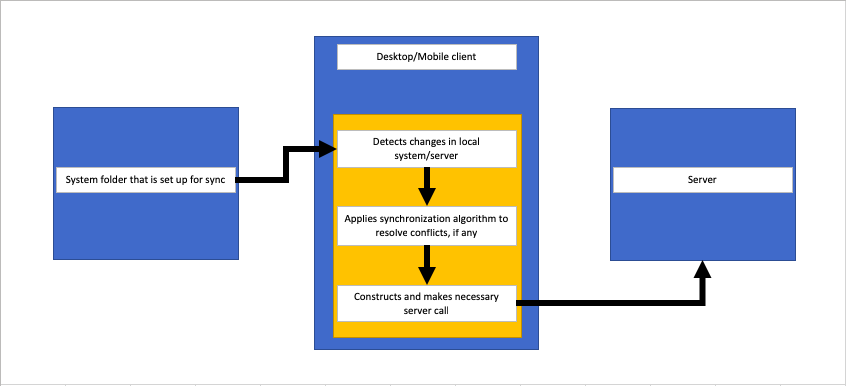
\includegraphics[width=\linewidth]{images/1.png}
	\caption{Flow of control between client and server}
\end{figure}\par
In our Agile workflow, we will start by building a basic prototype of the desktop client. This prototype will perform functionalities of Create, Edit, Rename and Delete for non-conflicting files for single user. It will also have a \emph{Upload} and \emph{Download} button to manually invoke synchronization. Then we will extend this prototype to handle conflict scenarios. The potential conflict scenarios and their resolution are stated in table \ref{table:conflict}.

Once the conflict resolution algorithm implementation is stable, we will develop the mobile client prototype followed by testing conflict resolution using mobile-desktop client pair. After satisfactory testing, we will move to the final phase of introducing automatic file sync using \emph{file system notification} and \emph{server polling}.

\begin{minipage}{\linewidth}
\centering
\captionof{table}{Conflict scenarios and resolutions} \label{table:conflict}
\begin{tabular}[H]{|C{0.75cm}|C{2.25cm}|C{2.25cm}|C{6cm}|}\toprule[1.5pt]
\bf No. & \bf Operation 1 & \bf Operation 2 & \bf Resolution\\\midrule
1       &  Create 	& Create     		&  \begin{flushleft}Upload both files, one with the original name and one with a prefix (eg. (1) or 'copy')\end{flushleft}\\\hline
2       &  Create   & Edit       		&  \begin{flushleft}Upload edit changes to the original file and upload new file with a prefix (eg. (1) or 'copy')\end{flushleft}\\\hline
3       &  Create   & Rename      		&  \begin{flushleft}Rename is applied first followed by upload of new file\end{flushleft}\\\hline
4       &  Create   & Delete     		&  \begin{flushleft}Delete file first and then upload the newly created file\end{flushleft}\\\hline
5       &  Edit		& Edit      		&  \begin{flushleft}Possible strategies: \begin{itemize} \item{Send server error for both requests} \item{Upload two copies of the file, each with different edits} \end{itemize}\end{flushleft}\\\hline
6       &  Edit		& Rename      		&  \begin{flushleft}Rename original file and upload document with edited changes as a new file\end{flushleft}\\\hline
7       &  Edit		& Delete      		&  \begin{flushleft}Delete original file and upload document with edited changes as a new file\end{flushleft}\\\hline
8       &  Rename   & Rename      		&  \begin{flushleft}Rename original file on server to name1 and upload another copy of the file with name2\end{flushleft}\\\hline
9       &  Rename   & Delete      		&  \begin{flushleft}Delete original file and upload another copy of the file with the new name\end{flushleft}\\\hline
10      &  Delete   & Delete      		&  \begin{flushleft}No conflict\end{flushleft}\\
\bottomrule[1.25pt]
\end {tabular}\par
\bigskip
\emph{Operation 1 and 2 are performed on/for files with the same name by same/different users from different devices.}
\end{minipage}
